%---------------------------------------------------------------------------
% Monitoring Hub component.
%
%---------------------------------------------------------------------------
\section{Monitoring Hub}
\label{sec:arch_monitoring_hub}

Monitoring Hub is the core component of the system. If using a layered model to analyze the application, the Monitoring Hub should be treated as a logic layer - placed between the presentation layer (GUI) and the data access layer (transport proxies). It provides services to GUI and it uses Transport Proxy implementations and Knowledge component. Its main responsibilities include: resource management (registering new resources, discovery dependent resources), measurement management (creation, pausing, resuming and termination) and the creation of scheduled jobs that polls for capability values and pushes new values to the registered listeners.

When user wants to start monitoring a new resource, he or she must choose which Monitoring Hub to use. This decision creates a direct association between the chosen hub, the resource to monitor and all its child resources discovered during registration. This association defines that the Monitoring Hub associated during the registration and the discovery will process all request calls related to a given resource.

To make high-level components loosely coupled, Monitoring Hub is not aware of details about other components. To be able to provide its services it uses transport proxies and knowledge components, but it interacts with them only using commonly known interfaces. Additionally it is not aware about the existence of GUI component at all. It just provide services by implementing the given interface, and it uses also common listener interfaces to notify about a variety of events.


\subsection{Decomposition of Monitoring Hub}

A further decomposition of Monitoring Hub can be found in Figure~\ref{fig:decomposition_mon_hub}. This module is composed of the following low-level components:

\begin{figure}[ht]
\centering
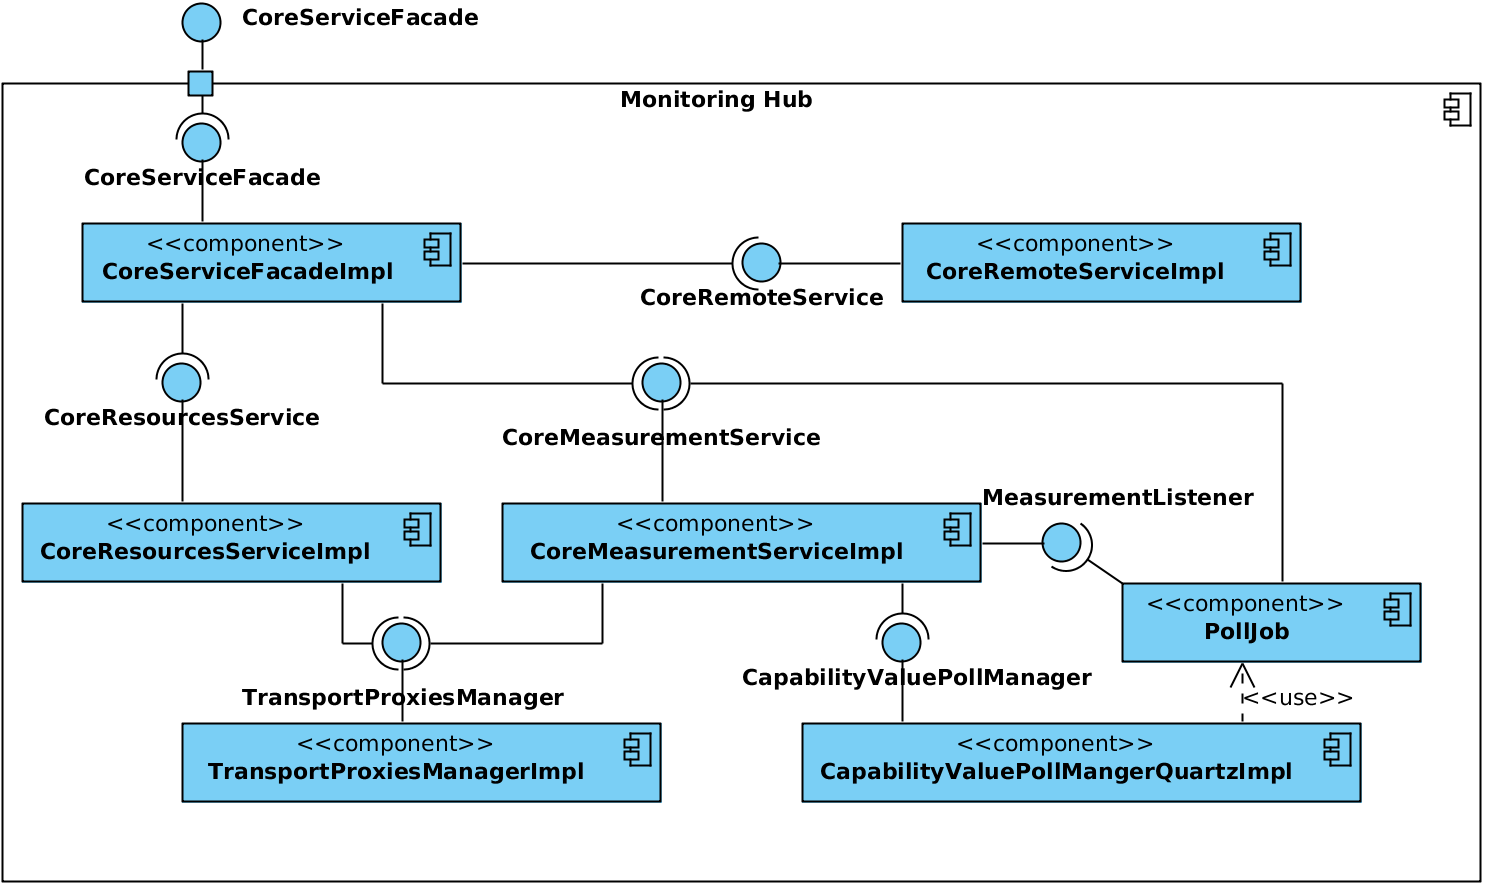
\includegraphics[width=0.9\textwidth]{decomposition_mon_hub}
\caption{Communication diagram - adding of new resource}
\label{fig:decomposition_mon_hub}
\end{figure}

\begin{itemize}

\item {\bf CoreServiceFacadeImpl}~~~~~~~~~~~~~~~~~~~~~~~~~~~~~~~~~~~~~~~~~~~~~~~~~~~~~~~~\linebreak
The \texttt{CoreServiceFacadeImpl} is a facade that allows access to all Monitoring Hub functionalities from a single interface. This wrapper eases remote access by exposing and using one interface with any remoting middle ware is easier than multiple ones. Having multiple interfaces in most cases would require multiple socket connections which can be a source of additional problems. We should tend to use as small amount connections as possible, because more connections system uses, the system becomes more and more prone to network configuration issues (e.g. firewalls). Additionally, the usage a single facade improves code style, as with facade, only a single interface has to be visible for all other components that are its clients.

\item {\bf CoreRemoteServiceImpl}~~~~~~~~~~~~~~~~~~~~~~~~~~~~~~~~~~~~~~~~~~~~~~~~~~~~~~~~\linebreak
The \texttt{CoreRemoteServiceImpl} is a service responsible for processing requests related to remote management of Monitoring Hub. It has two main responsibilities: it allows registering remote listening interfaces and it dispatches local events (new resource, new capability value etc.) to remote listeners in aggregated manner. Distributed dispatch of the events requires a bit different approach than the local one (local one, means dispatch inside of single JVM process). First of all, in most cases remote interface that will receive notifications with different signature, to allow handling exceptions related to networking. Additionally, to reduce the number of remote calls and thus improve efficiency, \texttt{CoreRemoteServiceImpl} aggregates events into batches and notifies remote listeners using a generated package of them. Such an approach does not distort measuring results, because each measurement value has associated a pickup timestamp (see~\ref{subsec:arch_comm_protocol}), initialized by the component that grabs given value, at the exact moment of the measurement. Additionally, as events related to resources addition/removal don\rq{}t require such a strict time association, those events can be aggregated without any issues.

\item {\bf CoreResourcesServiceImpl}~~~~~~~~~~~~~~~~~~~~~~~~~~~~~~~~~~~~~~~~~~~~~~~~~~~~~~~~\linebreak
The \texttt{CoreResourcesServiceImpl} is responsible for resource management: registering new resources, discovery of their children, returning all the registered and discovered ones. It is also used to get more details about a resource, like capabilities that the given resource may have.

\item {\bf CoreMeasurementServiceImpl}~~~~~~~~~~~~~~~~~~~~~~~~~~~~~~~~~~~~~~~~~~~~~~~~~~~~~~~~\linebreak
The \texttt{CoreMeasurementServiceImpl} can be used to create, pause, stop or terminate a measurement. Additionally it gathers the current values of capabilities. It is used by \texttt{PollJob} component for this purpose. It implements the \texttt{MeasurementListener} interface to be able to receive notifications about new capability values polled by \texttt{PollJob}. 

\item {\bf TransportProxiesManagerImpl}~~~~~~~~~~~~~~~~~~~~~~~~~~~~~~~~~~~~~~~~~~~~~~~~~~~~~~~~\linebreak
The \texttt{TransportProxiesManagerImpl} component manages the registered transport proxies. It is used by other components to get all transport proxies or to lookup a transport proxy that can be used to manage a given resource.

\item {\bf CapabilityValuePollManagerImpl}~~~~~~~~~~~~~~~~~~~~~~~~~~~~~~~~~~~~~~~~~~~~~~~~~~~~~~~~\linebreak
The \texttt{CapabilityValuePollManagerImpl} is responsible for managing jobs that poll for the capability values and are needed to run a measurement.

\item {\bf PollJob}~~~~~~~~~~~~~~~~~~~~~~~~~~~~~~~~~~~~~~~~~~~~~~~~~~~~~~~~\linebreak
A \texttt{PollJob} gets triggered a with a configured interval. It simply polls for a current capability value and push it to listeners specified during its creation.

\end{itemize}

\subsection{Most important data flows}

This section contains a description of the most salient data flows inside Monitoring Hub component. It covers the actions of adding new resources, adding new measurements, and dispatching a new capability value notification.

Figure~\ref{fig:comm_mh_add_res} depicts a communication diagram of adding new resources. In this scenario, external GUI component initiates an action - a \texttt{registerResource} request is the first step send by the external GUI component to the \texttt{CoreServiceFacadeImpl}. The facade simply delegates this call to \texttt{CoreResourcesServiceImpl} which will perform the actual registration. In the next step, \texttt{CoreResourcesServiceImpl} tries to find a proxy capable to communicate with a given resource by calling \texttt{TransportProxiesManagerImpl}. What should be noticed here, the Transport Proxy is an external component to the Monitoring Hub. After having successfully obtained a transport proxy, \texttt{CoreResourcesServiceImpl} performs a call to register the given resource. The registration here means a process needed by the Transport Proxy component to initialize the resource (and potentially itself) for further work with it. If this registration succeeds, the \texttt{CoreResourcesServiceImpl} uses the external Knowledge component, to get all types of child resources that the resource in subject may have. Using this list, the service requests \texttt{TransportProxy} to discover all children of the registered resource. After a successful discovery, notification containing the fully initialized resource is being dispatched to all listeners. This can be done either directly, when the given Monitoring Hub is embedded into the GUI or remotely, using the \texttt{CoreRemoteServiceImpl}.

\begin{figure}[ht]
\centering
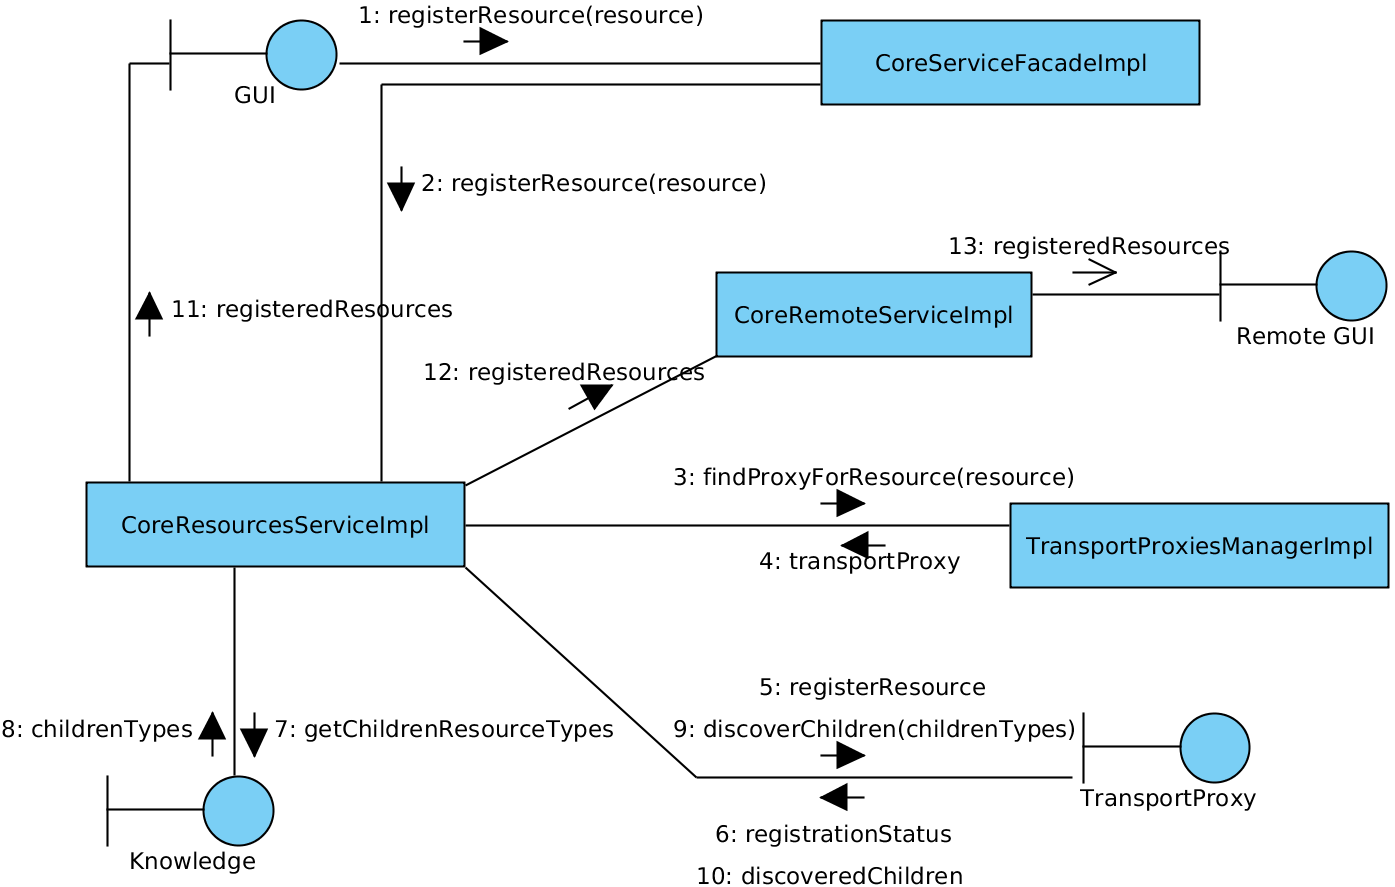
\includegraphics[width=0.9\textwidth]{comm_mh_add_res}
\caption{Monitoring Hub Communication diagram - adding new resource}
\label{fig:comm_mh_add_res}
\end{figure}

A communication diagram covering the action of adding new measurements can be found in Figure~\ref{fig:comm_mh_add_measurement}. In this scenario, again the GUI component is an initiator. The GUI component calls a \texttt{getResourceCapabilities} method; thus, sends the first request to \texttt{CoreServiceFacadeImpl}. Facade delegates query to \texttt{CoreResourcesServiceImpl}, which passes it to the external Knowledge component. A resulting list of capability URIs is being passed back, to the GUI component, which uses them to render a UI component that allows the user to choose which capability should be measured. On a selection event, the GUI requests \texttt{CoreServiceFacadeImpl} to create a measurement using the given definition (see Table~\ref{tab:TO_MeasurementDef}). Request is delegated to \texttt{CoreMeasurementServiceImpl} which is responsible for the creation of a measurement. The service requests \texttt{CapabilityValuePollManagerImpl} to create a new instance of the \texttt{PollJob} class. \texttt{CoreMeasurementServiceImpl} after creating a polling job, generates a measurement id, stores it internally with the measurement definition, and returns it to the requester. This identifier is then passed back to the GUI, which will use it in any future call referring the newly created measurement. Additionally it will be used to reference all incoming \texttt{CapabilityValue} objects.

\begin{figure}[ht]
\centering
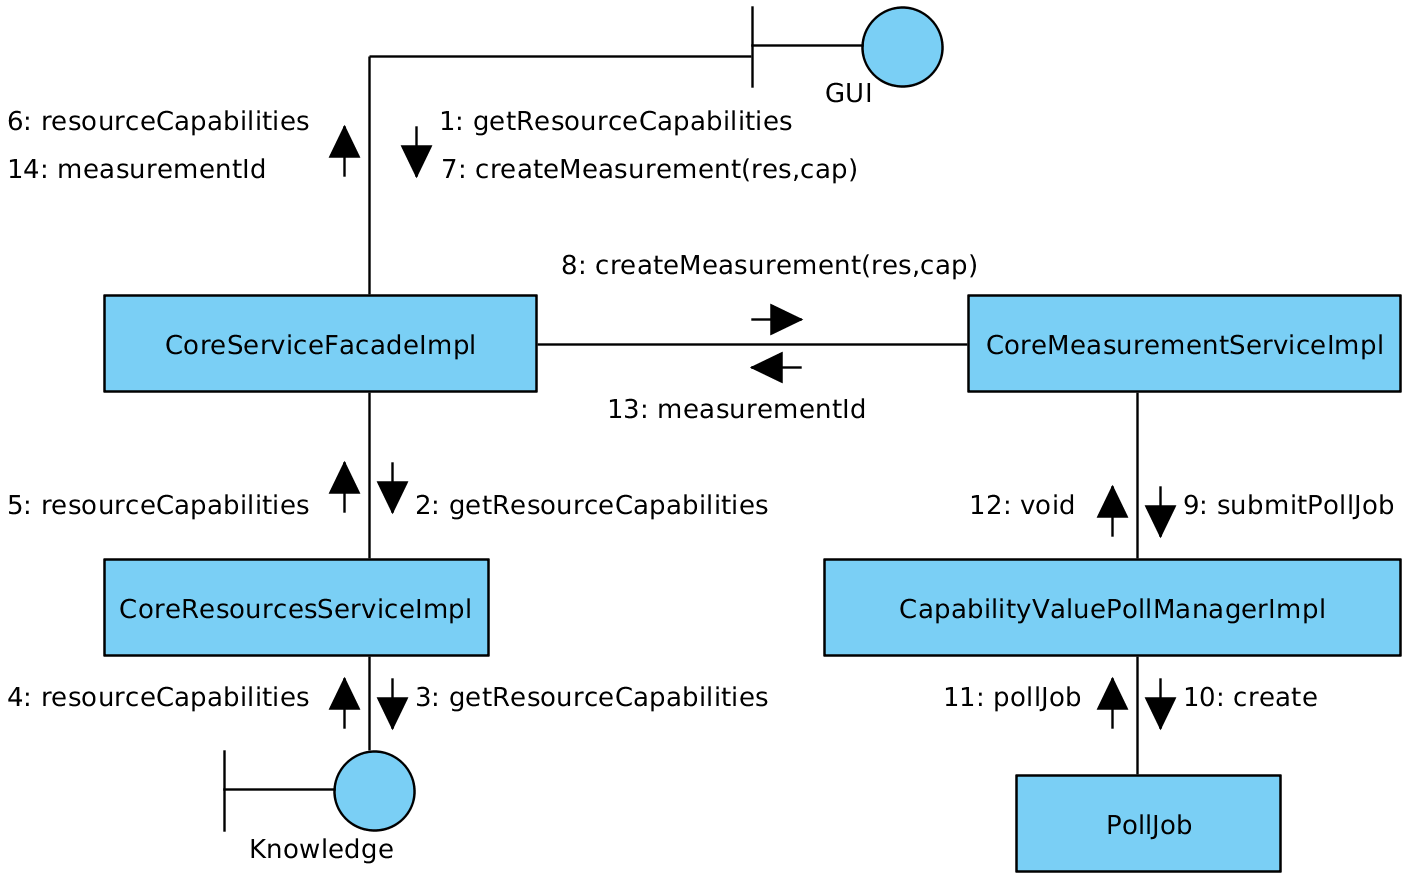
\includegraphics[width=0.8\textwidth]{comm_mh_add_measurement}
\caption{Communication diagram of adding new measurement}
\label{fig:comm_mh_add_measurement}
\end{figure}

The last data flow covered in this section describes gathering and publishing capability values. This time, the \texttt{CapabilityValuePollManagerImpl} initiates the action. Its internal scheduler triggers the previously created \texttt{PollJob} which contains the measurement definition (URI's of resource and capability). Using these identifiers, the \texttt{PollJob} calls the \texttt{CoreMeasurementServiceImpl} to get the capability value. The \texttt{CoreMeasurementServiceImpl} service first looks up the transport proxy using \texttt{TransportProxiesManagerImpl} and then, using the external Transport Proxy component, gets the capability value. In the subsequent step, the gathered capability value is being pushed to all listeners, either directly or using \texttt{CoreRemoteServiceImpl} to all remote listeners. What should be noticed here is that \texttt{CoreRemoteServiceImpl} notifies remote listeners in an asynchronous and aggregated manner.

\begin{figure}[ht]
\centering
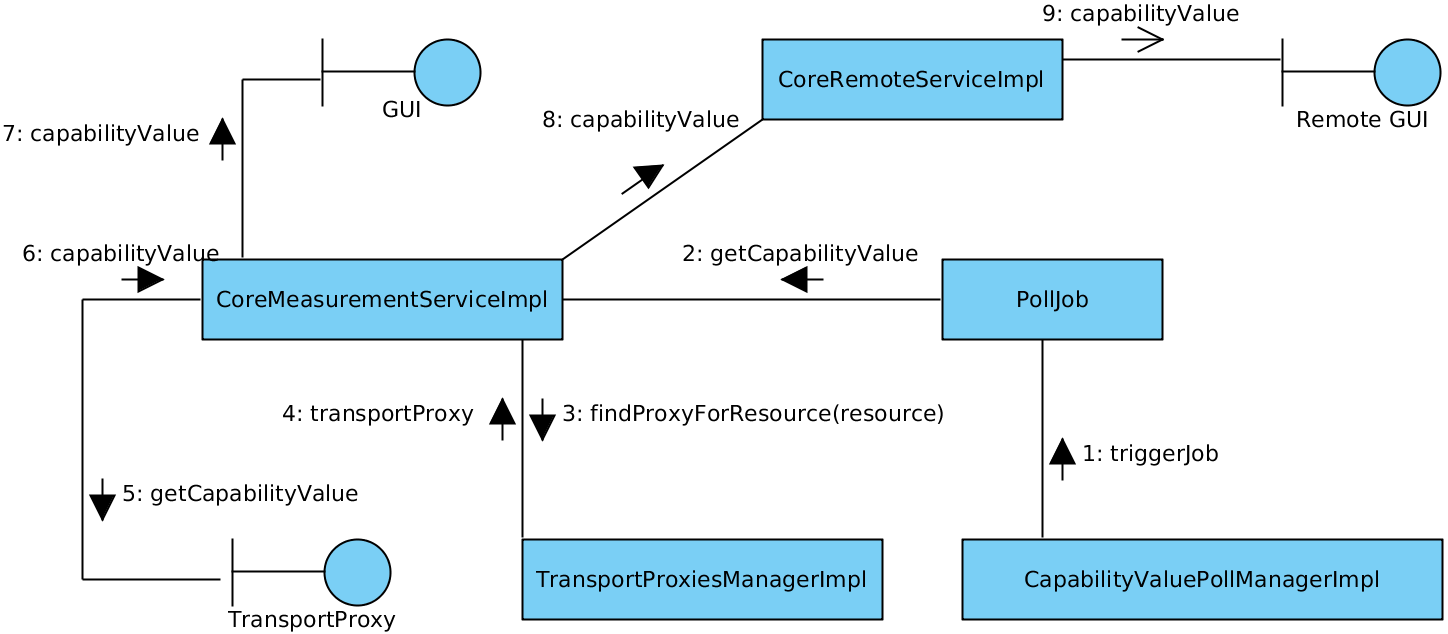
\includegraphics[width=1\textwidth]{comm_mh_new_cap_val}
\caption{Communication diagram of new capability value notification}
\label{fig:comm_new_cap_val}
\end{figure}
\pagebreak
